
% Default to the notebook output style

    


% Inherit from the specified cell style.




    
\documentclass[11pt]{article}

    
    
    \usepackage[T1]{fontenc}
    % Nicer default font (+ math font) than Computer Modern for most use cases
    \usepackage{mathpazo}
	\usepackage{float}
    % Basic figure setup, for now with no caption control since it's done
    % automatically by Pandoc (which extracts ![](path) syntax from Markdown).
    \usepackage{graphicx}
    % We will generate all images so they have a width \maxwidth. This means
    % that they will get their normal width if they fit onto the page, but
    % are scaled down if they would overflow the margins.
    \makeatletter
    \def\maxwidth{\ifdim\Gin@nat@width>\linewidth\linewidth
    \else\Gin@nat@width\fi}
    \makeatother
    \let\Oldincludegraphics\includegraphics
    % Set max figure width to be 80% of text width, for now hardcoded.
    \renewcommand{\includegraphics}[1]{\Oldincludegraphics[width=.8\maxwidth]{#1}}
    % Ensure that by default, figures have no caption (until we provide a
    % proper Figure object with a Caption API and a way to capture that
    % in the conversion process - todo).
    \usepackage{caption}
    \DeclareCaptionLabelFormat{nolabel}{}
    \captionsetup{labelformat=nolabel}

    \usepackage{adjustbox} % Used to constrain images to a maximum size 
    \usepackage{xcolor} % Allow colors to be defined
    \usepackage{enumerate} % Needed for markdown enumerations to work
    \usepackage{geometry} % Used to adjust the document margins
    \usepackage{amsmath} % Equations
    \usepackage{amssymb} % Equations
    \usepackage{textcomp} % defines textquotesingle
    % Hack from http://tex.stackexchange.com/a/47451/13684:
    \AtBeginDocument{%
        \def\PYZsq{\textquotesingle}% Upright quotes in Pygmentized code
    }
    \usepackage{upquote} % Upright quotes for verbatim code
    \usepackage{eurosym} % defines \euro
    \usepackage[mathletters]{ucs} % Extended unicode (utf-8) support
    \usepackage[utf8x]{inputenc} % Allow utf-8 characters in the tex document
    \usepackage{fancyvrb} % verbatim replacement that allows latex
    \usepackage{grffile} % extends the file name processing of package graphics 
                         % to support a larger range 
    % The hyperref package gives us a pdf with properly built
    % internal navigation ('pdf bookmarks' for the table of contents,
    % internal cross-reference links, web links for URLs, etc.)
    \usepackage{hyperref}
    \usepackage{longtable} % longtable support required by pandoc >1.10
    \usepackage{booktabs}  % table support for pandoc > 1.12.2
    \usepackage[inline]{enumitem} % IRkernel/repr support (it uses the enumerate* environment)
    \usepackage[normalem]{ulem} % ulem is needed to support strikethroughs (\sout)
                                % normalem makes italics be italics, not underlines
    

    
    
    % Colors for the hyperref package
    \definecolor{urlcolor}{rgb}{0,.145,.698}
    \definecolor{linkcolor}{rgb}{.71,0.21,0.01}
    \definecolor{citecolor}{rgb}{.12,.54,.11}

    % ANSI colors
    \definecolor{ansi-black}{HTML}{3E424D}
    \definecolor{ansi-black-intense}{HTML}{282C36}
    \definecolor{ansi-red}{HTML}{E75C58}
    \definecolor{ansi-red-intense}{HTML}{B22B31}
    \definecolor{ansi-green}{HTML}{00A250}
    \definecolor{ansi-green-intense}{HTML}{007427}
    \definecolor{ansi-yellow}{HTML}{DDB62B}
    \definecolor{ansi-yellow-intense}{HTML}{B27D12}
    \definecolor{ansi-blue}{HTML}{208FFB}
    \definecolor{ansi-blue-intense}{HTML}{0065CA}
    \definecolor{ansi-magenta}{HTML}{D160C4}
    \definecolor{ansi-magenta-intense}{HTML}{A03196}
    \definecolor{ansi-cyan}{HTML}{60C6C8}
    \definecolor{ansi-cyan-intense}{HTML}{258F8F}
    \definecolor{ansi-white}{HTML}{C5C1B4}
    \definecolor{ansi-white-intense}{HTML}{A1A6B2}

    % commands and environments needed by pandoc snippets
    % extracted from the output of `pandoc -s`
    \providecommand{\tightlist}{%
      \setlength{\itemsep}{0pt}\setlength{\parskip}{0pt}}
    \DefineVerbatimEnvironment{Highlighting}{Verbatim}{commandchars=\\\{\}}
    % Add ',fontsize=\small' for more characters per line
    \newenvironment{Shaded}{}{}
    \newcommand{\KeywordTok}[1]{\textcolor[rgb]{0.00,0.44,0.13}{\textbf{{#1}}}}
    \newcommand{\DataTypeTok}[1]{\textcolor[rgb]{0.56,0.13,0.00}{{#1}}}
    \newcommand{\DecValTok}[1]{\textcolor[rgb]{0.25,0.63,0.44}{{#1}}}
    \newcommand{\BaseNTok}[1]{\textcolor[rgb]{0.25,0.63,0.44}{{#1}}}
    \newcommand{\FloatTok}[1]{\textcolor[rgb]{0.25,0.63,0.44}{{#1}}}
    \newcommand{\CharTok}[1]{\textcolor[rgb]{0.25,0.44,0.63}{{#1}}}
    \newcommand{\StringTok}[1]{\textcolor[rgb]{0.25,0.44,0.63}{{#1}}}
    \newcommand{\CommentTok}[1]{\textcolor[rgb]{0.38,0.63,0.69}{\textit{{#1}}}}
    \newcommand{\OtherTok}[1]{\textcolor[rgb]{0.00,0.44,0.13}{{#1}}}
    \newcommand{\AlertTok}[1]{\textcolor[rgb]{1.00,0.00,0.00}{\textbf{{#1}}}}
    \newcommand{\FunctionTok}[1]{\textcolor[rgb]{0.02,0.16,0.49}{{#1}}}
    \newcommand{\RegionMarkerTok}[1]{{#1}}
    \newcommand{\ErrorTok}[1]{\textcolor[rgb]{1.00,0.00,0.00}{\textbf{{#1}}}}
    \newcommand{\NormalTok}[1]{{#1}}
    
    % Additional commands for more recent versions of Pandoc
    \newcommand{\ConstantTok}[1]{\textcolor[rgb]{0.53,0.00,0.00}{{#1}}}
    \newcommand{\SpecialCharTok}[1]{\textcolor[rgb]{0.25,0.44,0.63}{{#1}}}
    \newcommand{\VerbatimStringTok}[1]{\textcolor[rgb]{0.25,0.44,0.63}{{#1}}}
    \newcommand{\SpecialStringTok}[1]{\textcolor[rgb]{0.73,0.40,0.53}{{#1}}}
    \newcommand{\ImportTok}[1]{{#1}}
    \newcommand{\DocumentationTok}[1]{\textcolor[rgb]{0.73,0.13,0.13}{\textit{{#1}}}}
    \newcommand{\AnnotationTok}[1]{\textcolor[rgb]{0.38,0.63,0.69}{\textbf{\textit{{#1}}}}}
    \newcommand{\CommentVarTok}[1]{\textcolor[rgb]{0.38,0.63,0.69}{\textbf{\textit{{#1}}}}}
    \newcommand{\VariableTok}[1]{\textcolor[rgb]{0.10,0.09,0.49}{{#1}}}
    \newcommand{\ControlFlowTok}[1]{\textcolor[rgb]{0.00,0.44,0.13}{\textbf{{#1}}}}
    \newcommand{\OperatorTok}[1]{\textcolor[rgb]{0.40,0.40,0.40}{{#1}}}
    \newcommand{\BuiltInTok}[1]{{#1}}
    \newcommand{\ExtensionTok}[1]{{#1}}
    \newcommand{\PreprocessorTok}[1]{\textcolor[rgb]{0.74,0.48,0.00}{{#1}}}
    \newcommand{\AttributeTok}[1]{\textcolor[rgb]{0.49,0.56,0.16}{{#1}}}
    \newcommand{\InformationTok}[1]{\textcolor[rgb]{0.38,0.63,0.69}{\textbf{\textit{{#1}}}}}
    \newcommand{\WarningTok}[1]{\textcolor[rgb]{0.38,0.63,0.69}{\textbf{\textit{{#1}}}}}
    
    
    % Define a nice break command that doesn't care if a line doesn't already
    % exist.
    \def\br{\hspace*{\fill} \\* }
    % Math Jax compatability definitions
    \def\gt{>}
    \def\lt{<}
    % Document parameters
    \title{CMM201 Week 1}
    
    
    

    % Pygments definitions
    
\makeatletter
\def\PY@reset{\let\PY@it=\relax \let\PY@bf=\relax%
    \let\PY@ul=\relax \let\PY@tc=\relax%
    \let\PY@bc=\relax \let\PY@ff=\relax}
\def\PY@tok#1{\csname PY@tok@#1\endcsname}
\def\PY@toks#1+{\ifx\relax#1\empty\else%
    \PY@tok{#1}\expandafter\PY@toks\fi}
\def\PY@do#1{\PY@bc{\PY@tc{\PY@ul{%
    \PY@it{\PY@bf{\PY@ff{#1}}}}}}}
\def\PY#1#2{\PY@reset\PY@toks#1+\relax+\PY@do{#2}}

\expandafter\def\csname PY@tok@w\endcsname{\def\PY@tc##1{\textcolor[rgb]{0.73,0.73,0.73}{##1}}}
\expandafter\def\csname PY@tok@c\endcsname{\let\PY@it=\textit\def\PY@tc##1{\textcolor[rgb]{0.25,0.50,0.50}{##1}}}
\expandafter\def\csname PY@tok@cp\endcsname{\def\PY@tc##1{\textcolor[rgb]{0.74,0.48,0.00}{##1}}}
\expandafter\def\csname PY@tok@k\endcsname{\let\PY@bf=\textbf\def\PY@tc##1{\textcolor[rgb]{0.00,0.50,0.00}{##1}}}
\expandafter\def\csname PY@tok@kp\endcsname{\def\PY@tc##1{\textcolor[rgb]{0.00,0.50,0.00}{##1}}}
\expandafter\def\csname PY@tok@kt\endcsname{\def\PY@tc##1{\textcolor[rgb]{0.69,0.00,0.25}{##1}}}
\expandafter\def\csname PY@tok@o\endcsname{\def\PY@tc##1{\textcolor[rgb]{0.40,0.40,0.40}{##1}}}
\expandafter\def\csname PY@tok@ow\endcsname{\let\PY@bf=\textbf\def\PY@tc##1{\textcolor[rgb]{0.67,0.13,1.00}{##1}}}
\expandafter\def\csname PY@tok@nb\endcsname{\def\PY@tc##1{\textcolor[rgb]{0.00,0.50,0.00}{##1}}}
\expandafter\def\csname PY@tok@nf\endcsname{\def\PY@tc##1{\textcolor[rgb]{0.00,0.00,1.00}{##1}}}
\expandafter\def\csname PY@tok@nc\endcsname{\let\PY@bf=\textbf\def\PY@tc##1{\textcolor[rgb]{0.00,0.00,1.00}{##1}}}
\expandafter\def\csname PY@tok@nn\endcsname{\let\PY@bf=\textbf\def\PY@tc##1{\textcolor[rgb]{0.00,0.00,1.00}{##1}}}
\expandafter\def\csname PY@tok@ne\endcsname{\let\PY@bf=\textbf\def\PY@tc##1{\textcolor[rgb]{0.82,0.25,0.23}{##1}}}
\expandafter\def\csname PY@tok@nv\endcsname{\def\PY@tc##1{\textcolor[rgb]{0.10,0.09,0.49}{##1}}}
\expandafter\def\csname PY@tok@no\endcsname{\def\PY@tc##1{\textcolor[rgb]{0.53,0.00,0.00}{##1}}}
\expandafter\def\csname PY@tok@nl\endcsname{\def\PY@tc##1{\textcolor[rgb]{0.63,0.63,0.00}{##1}}}
\expandafter\def\csname PY@tok@ni\endcsname{\let\PY@bf=\textbf\def\PY@tc##1{\textcolor[rgb]{0.60,0.60,0.60}{##1}}}
\expandafter\def\csname PY@tok@na\endcsname{\def\PY@tc##1{\textcolor[rgb]{0.49,0.56,0.16}{##1}}}
\expandafter\def\csname PY@tok@nt\endcsname{\let\PY@bf=\textbf\def\PY@tc##1{\textcolor[rgb]{0.00,0.50,0.00}{##1}}}
\expandafter\def\csname PY@tok@nd\endcsname{\def\PY@tc##1{\textcolor[rgb]{0.67,0.13,1.00}{##1}}}
\expandafter\def\csname PY@tok@s\endcsname{\def\PY@tc##1{\textcolor[rgb]{0.73,0.13,0.13}{##1}}}
\expandafter\def\csname PY@tok@sd\endcsname{\let\PY@it=\textit\def\PY@tc##1{\textcolor[rgb]{0.73,0.13,0.13}{##1}}}
\expandafter\def\csname PY@tok@si\endcsname{\let\PY@bf=\textbf\def\PY@tc##1{\textcolor[rgb]{0.73,0.40,0.53}{##1}}}
\expandafter\def\csname PY@tok@se\endcsname{\let\PY@bf=\textbf\def\PY@tc##1{\textcolor[rgb]{0.73,0.40,0.13}{##1}}}
\expandafter\def\csname PY@tok@sr\endcsname{\def\PY@tc##1{\textcolor[rgb]{0.73,0.40,0.53}{##1}}}
\expandafter\def\csname PY@tok@ss\endcsname{\def\PY@tc##1{\textcolor[rgb]{0.10,0.09,0.49}{##1}}}
\expandafter\def\csname PY@tok@sx\endcsname{\def\PY@tc##1{\textcolor[rgb]{0.00,0.50,0.00}{##1}}}
\expandafter\def\csname PY@tok@m\endcsname{\def\PY@tc##1{\textcolor[rgb]{0.40,0.40,0.40}{##1}}}
\expandafter\def\csname PY@tok@gh\endcsname{\let\PY@bf=\textbf\def\PY@tc##1{\textcolor[rgb]{0.00,0.00,0.50}{##1}}}
\expandafter\def\csname PY@tok@gu\endcsname{\let\PY@bf=\textbf\def\PY@tc##1{\textcolor[rgb]{0.50,0.00,0.50}{##1}}}
\expandafter\def\csname PY@tok@gd\endcsname{\def\PY@tc##1{\textcolor[rgb]{0.63,0.00,0.00}{##1}}}
\expandafter\def\csname PY@tok@gi\endcsname{\def\PY@tc##1{\textcolor[rgb]{0.00,0.63,0.00}{##1}}}
\expandafter\def\csname PY@tok@gr\endcsname{\def\PY@tc##1{\textcolor[rgb]{1.00,0.00,0.00}{##1}}}
\expandafter\def\csname PY@tok@ge\endcsname{\let\PY@it=\textit}
\expandafter\def\csname PY@tok@gs\endcsname{\let\PY@bf=\textbf}
\expandafter\def\csname PY@tok@gp\endcsname{\let\PY@bf=\textbf\def\PY@tc##1{\textcolor[rgb]{0.00,0.00,0.50}{##1}}}
\expandafter\def\csname PY@tok@go\endcsname{\def\PY@tc##1{\textcolor[rgb]{0.53,0.53,0.53}{##1}}}
\expandafter\def\csname PY@tok@gt\endcsname{\def\PY@tc##1{\textcolor[rgb]{0.00,0.27,0.87}{##1}}}
\expandafter\def\csname PY@tok@err\endcsname{\def\PY@bc##1{\setlength{\fboxsep}{0pt}\fcolorbox[rgb]{1.00,0.00,0.00}{1,1,1}{\strut ##1}}}
\expandafter\def\csname PY@tok@kc\endcsname{\let\PY@bf=\textbf\def\PY@tc##1{\textcolor[rgb]{0.00,0.50,0.00}{##1}}}
\expandafter\def\csname PY@tok@kd\endcsname{\let\PY@bf=\textbf\def\PY@tc##1{\textcolor[rgb]{0.00,0.50,0.00}{##1}}}
\expandafter\def\csname PY@tok@kn\endcsname{\let\PY@bf=\textbf\def\PY@tc##1{\textcolor[rgb]{0.00,0.50,0.00}{##1}}}
\expandafter\def\csname PY@tok@kr\endcsname{\let\PY@bf=\textbf\def\PY@tc##1{\textcolor[rgb]{0.00,0.50,0.00}{##1}}}
\expandafter\def\csname PY@tok@bp\endcsname{\def\PY@tc##1{\textcolor[rgb]{0.00,0.50,0.00}{##1}}}
\expandafter\def\csname PY@tok@fm\endcsname{\def\PY@tc##1{\textcolor[rgb]{0.00,0.00,1.00}{##1}}}
\expandafter\def\csname PY@tok@vc\endcsname{\def\PY@tc##1{\textcolor[rgb]{0.10,0.09,0.49}{##1}}}
\expandafter\def\csname PY@tok@vg\endcsname{\def\PY@tc##1{\textcolor[rgb]{0.10,0.09,0.49}{##1}}}
\expandafter\def\csname PY@tok@vi\endcsname{\def\PY@tc##1{\textcolor[rgb]{0.10,0.09,0.49}{##1}}}
\expandafter\def\csname PY@tok@vm\endcsname{\def\PY@tc##1{\textcolor[rgb]{0.10,0.09,0.49}{##1}}}
\expandafter\def\csname PY@tok@sa\endcsname{\def\PY@tc##1{\textcolor[rgb]{0.73,0.13,0.13}{##1}}}
\expandafter\def\csname PY@tok@sb\endcsname{\def\PY@tc##1{\textcolor[rgb]{0.73,0.13,0.13}{##1}}}
\expandafter\def\csname PY@tok@sc\endcsname{\def\PY@tc##1{\textcolor[rgb]{0.73,0.13,0.13}{##1}}}
\expandafter\def\csname PY@tok@dl\endcsname{\def\PY@tc##1{\textcolor[rgb]{0.73,0.13,0.13}{##1}}}
\expandafter\def\csname PY@tok@s2\endcsname{\def\PY@tc##1{\textcolor[rgb]{0.73,0.13,0.13}{##1}}}
\expandafter\def\csname PY@tok@sh\endcsname{\def\PY@tc##1{\textcolor[rgb]{0.73,0.13,0.13}{##1}}}
\expandafter\def\csname PY@tok@s1\endcsname{\def\PY@tc##1{\textcolor[rgb]{0.73,0.13,0.13}{##1}}}
\expandafter\def\csname PY@tok@mb\endcsname{\def\PY@tc##1{\textcolor[rgb]{0.40,0.40,0.40}{##1}}}
\expandafter\def\csname PY@tok@mf\endcsname{\def\PY@tc##1{\textcolor[rgb]{0.40,0.40,0.40}{##1}}}
\expandafter\def\csname PY@tok@mh\endcsname{\def\PY@tc##1{\textcolor[rgb]{0.40,0.40,0.40}{##1}}}
\expandafter\def\csname PY@tok@mi\endcsname{\def\PY@tc##1{\textcolor[rgb]{0.40,0.40,0.40}{##1}}}
\expandafter\def\csname PY@tok@il\endcsname{\def\PY@tc##1{\textcolor[rgb]{0.40,0.40,0.40}{##1}}}
\expandafter\def\csname PY@tok@mo\endcsname{\def\PY@tc##1{\textcolor[rgb]{0.40,0.40,0.40}{##1}}}
\expandafter\def\csname PY@tok@ch\endcsname{\let\PY@it=\textit\def\PY@tc##1{\textcolor[rgb]{0.25,0.50,0.50}{##1}}}
\expandafter\def\csname PY@tok@cm\endcsname{\let\PY@it=\textit\def\PY@tc##1{\textcolor[rgb]{0.25,0.50,0.50}{##1}}}
\expandafter\def\csname PY@tok@cpf\endcsname{\let\PY@it=\textit\def\PY@tc##1{\textcolor[rgb]{0.25,0.50,0.50}{##1}}}
\expandafter\def\csname PY@tok@c1\endcsname{\let\PY@it=\textit\def\PY@tc##1{\textcolor[rgb]{0.25,0.50,0.50}{##1}}}
\expandafter\def\csname PY@tok@cs\endcsname{\let\PY@it=\textit\def\PY@tc##1{\textcolor[rgb]{0.25,0.50,0.50}{##1}}}

\def\PYZbs{\char`\\}
\def\PYZus{\char`\_}
\def\PYZob{\char`\{}
\def\PYZcb{\char`\}}
\def\PYZca{\char`\^}
\def\PYZam{\char`\&}
\def\PYZlt{\char`\<}
\def\PYZgt{\char`\>}
\def\PYZsh{\char`\#}
\def\PYZpc{\char`\%}
\def\PYZdl{\char`\$}
\def\PYZhy{\char`\-}
\def\PYZsq{\char`\'}
\def\PYZdq{\char`\"}
\def\PYZti{\char`\~}
% for compatibility with earlier versions
\def\PYZat{@}
\def\PYZlb{[}
\def\PYZrb{]}
\makeatother


    % Exact colors from NB
    \definecolor{incolor}{rgb}{0.0, 0.0, 0.5}
    \definecolor{outcolor}{rgb}{0.545, 0.0, 0.0}



    
    % Prevent overflowing lines due to hard-to-break entities
    \sloppy 
    % Setup hyperref package
    \hypersetup{
      breaklinks=true,  % so long urls are correctly broken across lines
      colorlinks=true,
      urlcolor=urlcolor,
      linkcolor=linkcolor,
      citecolor=citecolor,
      }
    % Slightly bigger margins than the latex defaults
    
    \geometry{verbose,tmargin=1in,bmargin=1in,lmargin=1in,rmargin=1in}
    
    
	\date{}
    \begin{document}
    
    
    \maketitle
    

    \hypertarget{cmm201---programming-concepts-for-business-analytics}{%
\section{CMM201 - Programming Concepts for Business
Analytics}\label{cmm201---programming-concepts-for-business-analytics}}

\begin{itemize}
\tightlist
\item
  Dr.~Carlos Moreno-Garcia
\item
  Lecturer in Computing
\item
  Placements and Electives Coordinator
\item
  School of Computing Science and Digital Media
\end{itemize}

    \hypertarget{aim-of-the-module}{%
\subsection{Aim of the Module}\label{aim-of-the-module}}

This module will introduce students to fundamental programming
principles and concepts within the context of creating solutions for
business analytics.

    \hypertarget{learning-outcomes}{%
\subsection{Learning Outcomes}\label{learning-outcomes}}

On completion of this module, students are expected to be able to: 1.
Critically appraise a range of programming languages and tools commonly
used for data analytics (in this case, we will resort to the Python
programming language). 2. Demonstrate a critical understanding of core
programming techniques and concepts. 3. Use existing libraries and
coding techniques to perform data management, data analysis and data
visualization tasks. 4. Apply programming skills to business decision
making problems.

    \hypertarget{module-evaluation} of the
final mark: * First output: \textbf{7th November, 2019} * Second output:
\textbf{12th December, 2019}

The guidelines and submission instructions can be found
\href{http://campusmoodle.rgu.ac.uk/course/view.php?id=96406}{here}.

    \hypertarget{industry-partnershipengagement}{%
\subsection{Industry
Partnership/Engagement}\label{industry-partnershipengagement}}

Students are intended to learn basic programming knowledge and thus, the
engagement with industry is expected to be developed in the follow-up
module ``CMM202 -- Programming for Business Analytics''.

    \hypertarget{bibliography}{%
\section{Bibliography}\label{bibliography}}

    \hypertarget{books}{%
\subsection{Books}\label{books}}

\begin{itemize}
\tightlist
\item
  Python. Toby Donaldson, Peachpit Press, 2013.
\item
  Python Essentials. Steven F. Lott, Packt Publishing Ltd, 2015.
\item
  Think Python: How to Think Like a Computer Scientist. Allen Downey,
  O'Reilly Media, Inc., 2012.
\item
  Fluent Python. Luciano Ramalho. O'Reilly Media, Inc., 2015.
\item
  Python Cookbook: Recipes for Mastering Python 3. David Beazley, Brian
  K. Jones, O'Reilly Media, Inc., 10 May 2013.
\item
  Introduction to Computing and Programming in Python: A Multimedia
  Approach. Mark Guzdial, Barbara Ericson. Pearson, 2016.
\item
  Search the RGU Library in
  \href{https://librarysearch.rgu.ac.uk/discovery/search?query=any,contains,python\&tab=Everything\&search_scope=MyInst_and_CI\&vid=44RGU_INST:VU1\&offset=0}{here}.
\end{itemize}

    \hypertarget{podcasts}{%
\subsection{Podcasts}\label{podcasts}}

\begin{itemize}
\tightlist
\item
  https://talkpython.fm/
\item
  https://www.pythonpodcast.com/
\item
  https://testandcode.com/
\end{itemize}

    \hypertarget{websites}{%
\subsection{Websites}\label{websites}}

\begin{itemize}
\tightlist
\item
  \href{https://docs.python.org/3/}{Python Documentation}
\item
  \href{https://stackoverflow.com/questions/tagged/python}{StackOverflow}

  \begin{itemize}
  \tightlist
  \item
    Online community where people exchange ideas, doubts and code.
  \end{itemize}
\item
  \href{https://github.com/python}{Github} code repository.
\end{itemize}

    \hypertarget{online-courses}{%
\subsection{Online Courses}\label{online-courses}}

\begin{itemize}
\tightlist
\item
  \href{https://www.datacamp.com/courses/intro-to-python-for-data-science?utm_source=adwords_ppc\&utm_campaignid=805200711\&utm_adgroupid=43370829484\&utm_device=c\&utm_keyword=\%2Bdatacamp\%20\%2Bpython\&utm_matchtype=b\&utm_network=g\&utm_adpostion=1t1\&utm_creative=191104999116\&utm_targetid=kwd-414126611260\&utm_loc_interest_ms=\&utm_loc_physical_ms=9046834\&gclid=CjwKCAjw7_rlBRBaEiwAc23rhjfi2Mw2qxQ1_zJmVEph39YX5t6HkFUTmp48oqIpZ51eN2SYDpBPahoCqGEQAvD_BwE}{Datacamp}
  (you can also download the mobile app to practice on the go)
\item
  \href{www.codeinstitute.net}{CodeInstitute}
\item
  \href{https://www.learnpython.org/}{LearnPython} (free course)
\item
  \href{https://www.edx.org/learn/python}{EDX}
\item
  \href{https://www.coursera.org/courses?query=python}{Coursera}
\item
  \href{https://www.codecademy.com/learn/learn-python}{CodeAcademy}
\item
  \href{https://www.udemy.com/python-for-finance-investment-fundamentals-data-analytics/}{Udemy}
  Python for Finance: Investment Fundamentals \& Data Analytics.
\end{itemize}

    \hypertarget{events-in-the-city}{%
\subsection{Events in the City}\label{events-in-the-city}}

\begin{itemize}
\tightlist
\item
  Aberdeen Data Meetup (1st Tuesday of each month).

  \begin{itemize}
  \tightlist
  \item
    Organised by Scotland Data Science \& Technology Meetup group.
  \item
    Attendance managed through
    \href{https://www.meetup.com/Scotland-Data-Science-Technology-Meetup/}{Meetup}.
  \item
    Discussion about latest news, projects and needs of the city, all
    disciplines welcome.
  \end{itemize}
\item
  Python Aberdeen Group (2nd Wednesday of each month).

  \begin{itemize}
  \tightlist
  \item
    Organised by \href{https://codethecity.org/}{Code the City
    Aberdeen}.

    \begin{itemize}
    \tightlist
    \item
      They organise other events as well such as hackathons and
      workshops.
    \end{itemize}
  \item
    Attendance managed through
    \href{https://ti.to/code-the-city/}{Tito}.
  \end{itemize}
\end{itemize}

    \hypertarget{why-do-you-need-python}{%
\section{Why do you Need Python?}\label{why-do-you-need-python}}

\href{https://www.datacamp.com/community/blog/why-your-company-needs-python-for-business-analytics}{Source}

    \hypertarget{improves-work-for-everyone}{%
\subsection{Improves Work for
Everyone}\label{improves-work-for-everyone}}

\begin{itemize}
\tightlist
\item
  Widely used top programming language
\item
  Huge growing ecosystem due to its open source nature
\item
  Almost every industry is on board
\end{itemize}

    \hypertarget{is-replacing-excel}{%
\subsection{Is Replacing Excel}\label{is-replacing-excel}}

\begin{itemize}
\tightlist
\item
  Excel isn't scalable for modern business needs
\item
  Allows collaboration
\end{itemize}

    \hypertarget{descriptive-analytics-and-dashboards}{%
\subsection{Descriptive Analytics and
Dashboards}\label{descriptive-analytics-and-dashboards}}

\begin{itemize}
\tightlist
\item
  Exploratory Data Analysis
\item
  Manipulation of data
\item
  Streamline work flows
\item
  Creating visualisations
\end{itemize}

    \begin{figure}[H]
\centering
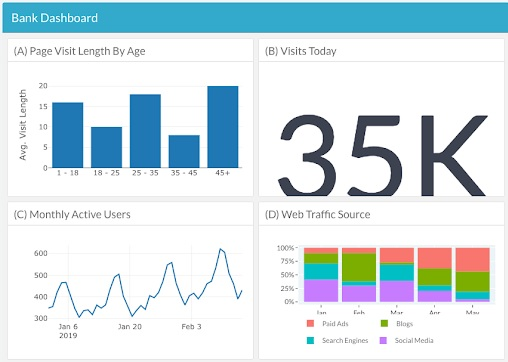
\includegraphics{figs/dashboard.jpg}
\caption{Fig. 1. Example of a dashboard in Python}
\end{figure}

    \hypertarget{machine-learning}{%
\subsection{Machine Learning}\label{machine-learning}}

\begin{itemize}
\tightlist
\item
  Predicting and classifying new data
\item
  Recommender systems
\item
  Can work with popular Google machine learning libraries (such as
  Tesseract and Tensorflow)
\end{itemize}

    \hypertarget{predictiveprescriptive-analytics}{%
\subsection{Predictive/Prescriptive
Analytics}\label{predictiveprescriptive-analytics}}

\begin{itemize}
\tightlist
\item
  Decision science

  \begin{itemize}
  \tightlist
  \item
    Anticipate what, when and why certain outcome will happen
  \item
    What to do with information
  \end{itemize}
\item
  Deep learning to optimise outcomes
\end{itemize}

    \begin{figure}[H]
\centering
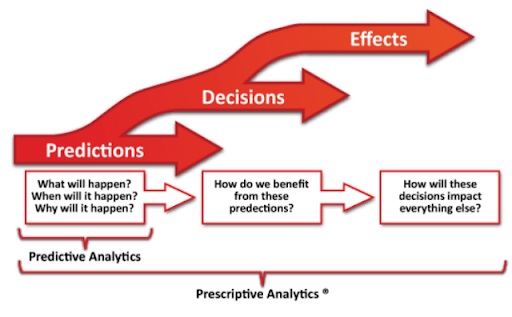
\includegraphics{figs/prescriptive.jpg}
\caption{Fig. 2. Prescriptive Analytics}
\end{figure}

    \hypertarget{fundamentals-of-programming}{%
\section{Fundamentals of
Programming}\label{fundamentals-of-programming}}

    \hypertarget{types-of-programming-languages}{%
\subsection{Types of Programming
Languages}\label{types-of-programming-languages}}

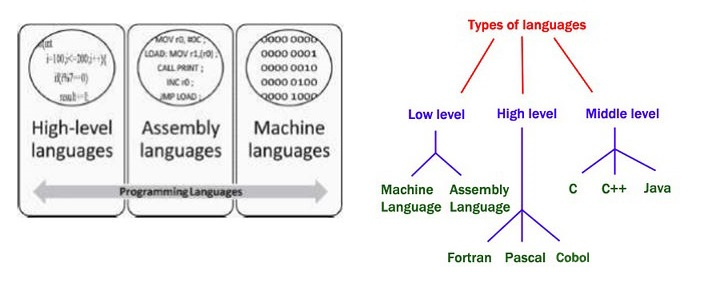
\includegraphics{figs/proglangtypes.jpg}
\href{http://4.bp.blogspot.com/-NvijJmjC13I/TmIbqlKKl8I/AAAAAAAAA3Q/mK4Nmy43en8/s1600/Untitled-1+\%25281\%2529.jpg}{Source
1}
\href{https://studyin24.com/wp-content/uploads/2018/12/Programming-language-types.jpg}{Source
2}

    \hypertarget{advantages-of-high-level-programming-languages}{%
\subsection{Advantages of High-level Programming
Languages}\label{advantages-of-high-level-programming-languages}}

\begin{itemize}
\tightlist
\item
  Programmer friendly.
\item
  Easy to write, debug and maintain.
\item
  Provide higher level of abstraction from machine languages.
\item
  Machine independent language.
\item
  Easy to learn.
\item
  Less error prone.
\item
  Results in better programming productivity.
\end{itemize}

    \hypertarget{compiled-vs-interpreted-programming-languages}{%
\subsection{Compiled vs Interpreted Programming
Languages}\label{compiled-vs-interpreted-programming-languages}}

    \hypertarget{compiled}{%
\subsubsection{Compiled}\label{compiled}}

\begin{itemize}
\tightlist
\item
  The high-level source code is translated to machine code using a
  compiler.
\item
  Example: An addition + gets directly translated to the ADD instruction
  in the machine code.
\item
  Examples: C, Fortran, COBOL, C++, and Java (compiled to bytecode).
\item
  Advantages:

  \begin{itemize}
  \tightlist
  \item
    Ready to run.
  \item
    Often faster.
  \item
    Source code is kept private.
  \end{itemize}
\end{itemize}

    \hypertarget{interpreted}{%
\subsubsection{Interpreted}\label{interpreted}}

\begin{itemize}
\tightlist
\item
  Instructions are not directly executed, but read by another program.
\item
  Instructions run freely without the need to compile them first!
\item
  Examples: JavaScript, Perl, R, \emph{Python}.
\item
  Advantages:

  \begin{itemize}
  \tightlist
  \item
    Cross-platform (portability).
  \item
    Simpler to test.
  \item
    Display error as each instruction is run.
  \end{itemize}
\end{itemize}

    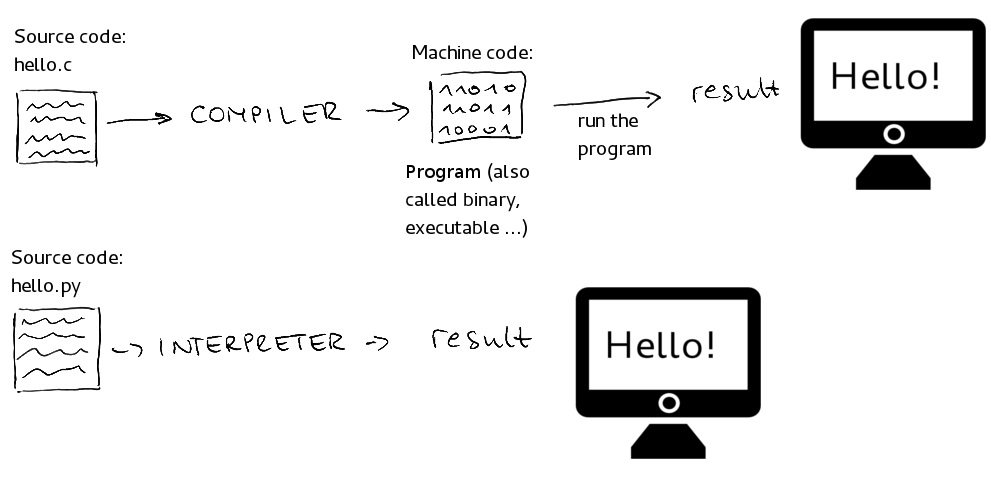
\includegraphics{figs/compiledinterpreted.jpg}
\href{https://www.google.com/url?sa=i\&rct=j\&q=\&esrc=s\&source=images\&cd=\&cad=rja\&uact=8\&ved=2ahUKEwichoGF1KXkAhVOdhoKHebmAJwQjRx6BAgBEAQ\&url=\%2Furl\%3Fsa\%3Di\%26rct\%3Dj\%26q\%3D\%26esrc\%3Ds\%26source\%3Dimages\%26cd\%3D\%26ved\%3D\%26url\%3Dhttps\%253A\%252F\%252Fmedium.com\%252Ffrom-the-scratch\%252Fstop-it-there-are-no-compiled-and-interpreted-languages-512f84756664\%26psig\%3DAOvVaw0CqS9Nmdo4wbc9J-p4WtL-\%26ust\%3D1567083827896505\&psig=AOvVaw0CqS9Nmdo4wbc9J-p4WtL-\&ust=1567083827896505}{Source}

    \hypertarget{static-vs-dynamic-programming-languages}{%
\subsection{Static vs Dynamic Programming
Languages}\label{static-vs-dynamic-programming-languages}}

\begin{itemize}
\tightlist
\item
  Static is designed to optimise \emph{hardware} efficiency
\item
  Dynamic is designed to optimise \emph{programming} efficiency so that
  less code is used.
\item
  In fact, dynamic languages are written using a static one.

  \begin{itemize}
  \tightlist
  \item
    Python is written in C!
  \end{itemize}
\end{itemize}

    \hypertarget{python}{%
\section{Python}\label{python}}

    \hypertarget{what-is-python}{%
\subsection{What is Python?}\label{what-is-python}}

\begin{itemize}
\tightlist
\item
  Widely used \textbf{high-level}, \textbf{interpreted},
  \textbf{dynamic} programming language.
\item
  Emphasizes code readability.
\item
  Its syntax allows programmers to express concepts in fewer lines of
  code.
\item
  Similar to R and Matlab.
\end{itemize}

    \hypertarget{some-statistics}{%
\subsection{Some statistics}\label{some-statistics}}

    \hypertarget{popularity}{%
\subsubsection{Popularity}\label{popularity}}

    Python is the third most popular programming language according to the
\href{https://www.tiobe.com/tiobe-index/}{TIOBE} index, being the
fastest growing one in this rubric for the current year.

    \begin{figure}[H]
\centering
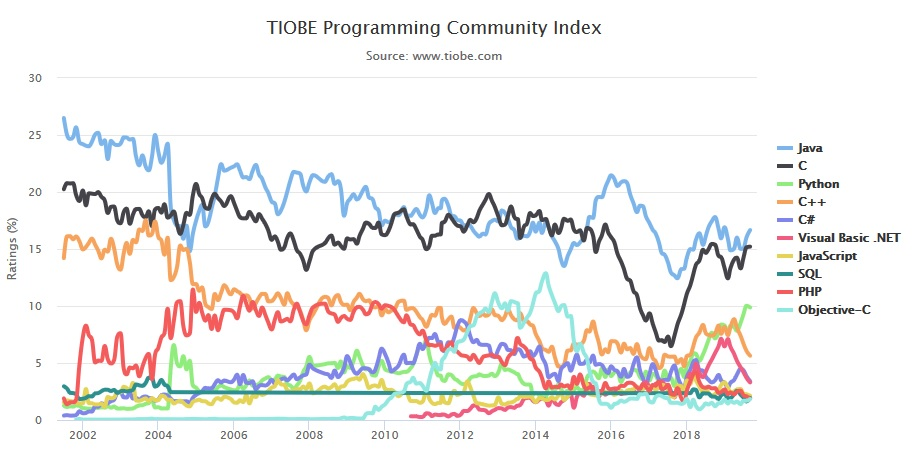
\includegraphics{figs/tiobe.jpg}
\caption{Fig. 5 a. TIOBE Index 2019}
\end{figure}

    \begin{figure}[H]
\centering
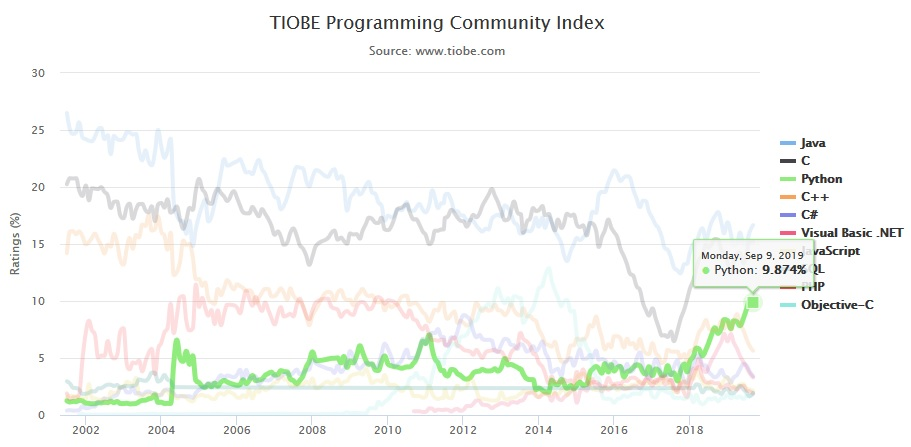
\includegraphics{figs/tiobepython.jpg}
\caption{Fig. 5 b. TIOBE Index 2019}
\end{figure}

    According to the 2019 developer survey run by
\href{https://insights.stackoverflow.com/survey/2019}{Stack overflow},
Python is the 4th most popular programming language in the world, both
for general public and for professional developers.

    \begin{figure}[H]
\centering
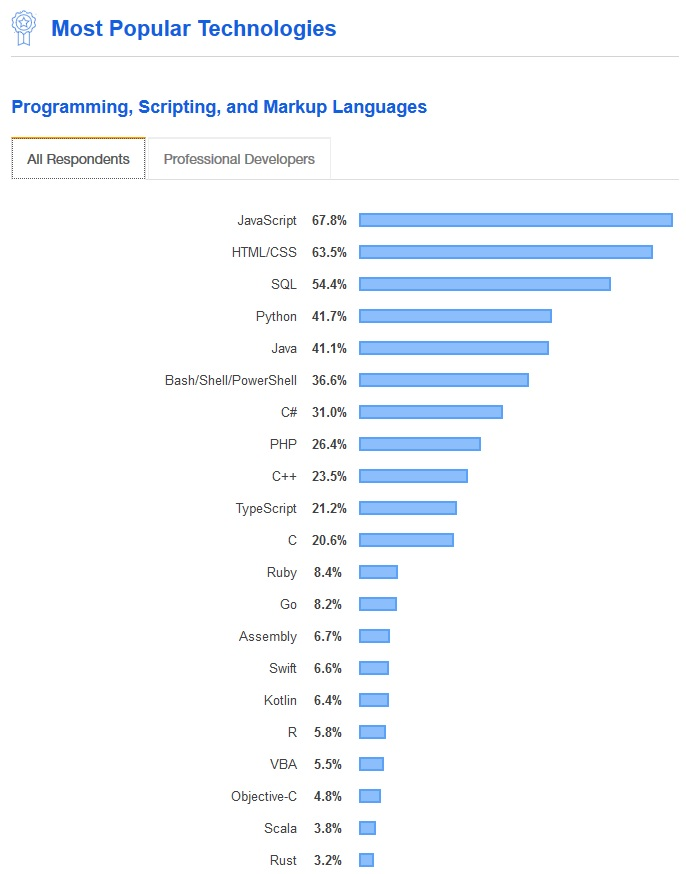
\includegraphics{figs/stackoverflowmostpopular.jpg}
\caption{Fig. 6. Most popular technologies}
\end{figure}

    Python is currently the best ranked programming language according to
the Institute of Electrical and Electronics Engineers
\href{https://spectrum.ieee.org/at-work/innovation/the-2018-top-programming-languages}{(IEEE)}.

    \begin{figure}[H]
\centering
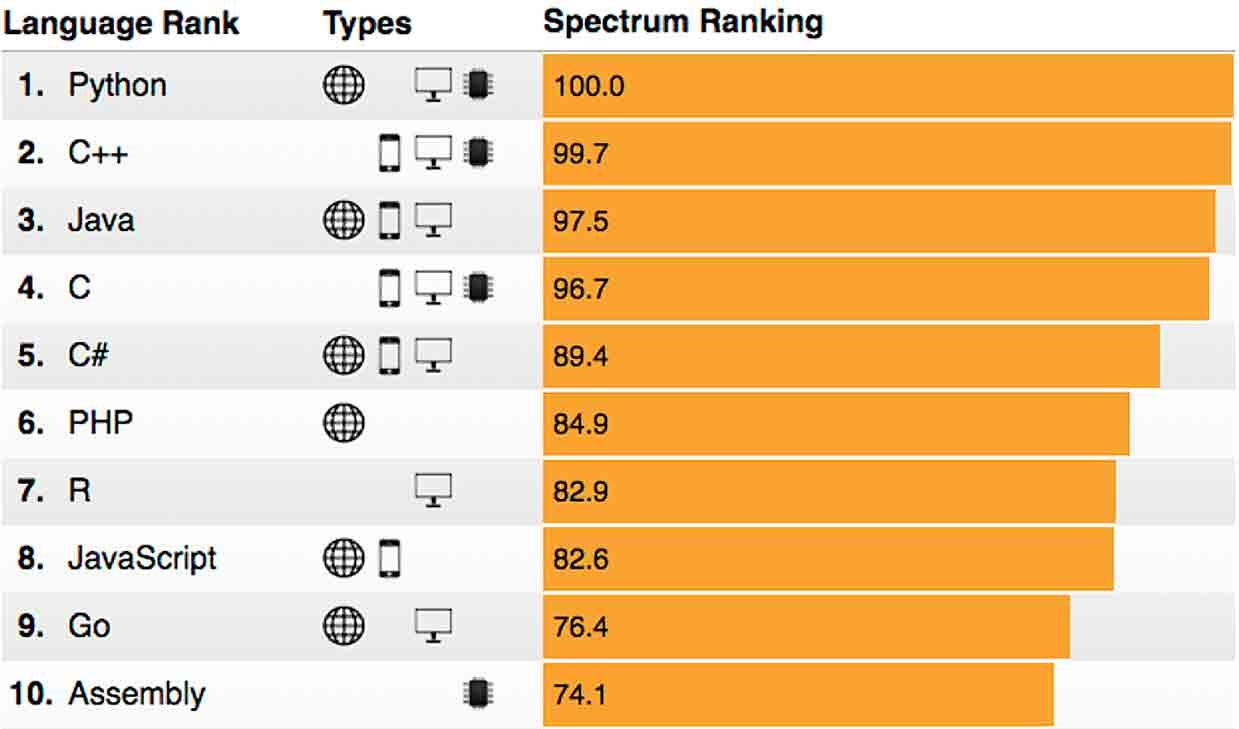
\includegraphics{figs/stats3.jpg}
\caption{Fig 7. IEEE Ranking}
\end{figure}

    \hypertarget{employabilty}{%
\subsubsection{Employabilty}\label{employabilty}}

    Python is currently the language with the fastest growing rate of
interest by employers according to
\href{https://medium.freecodecamp.org/best-programming-languages-to-learn-in-2018-ultimate-guide-bfc93e615b35}{Google
Trends}.

    \begin{figure}[H]
\centering
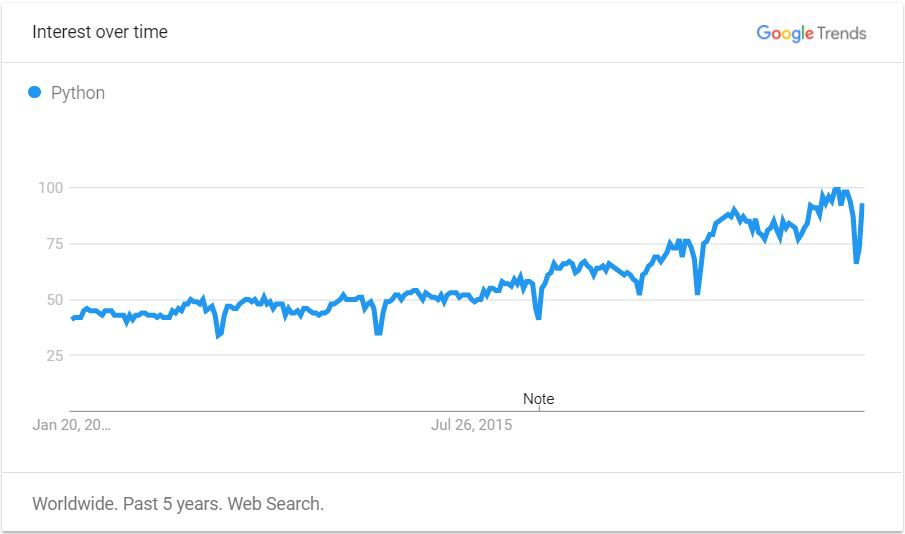
\includegraphics{figs/stats2.jpg}
\caption{Fig. 8. Google trends interest over time}
\end{figure}

    It is the 12th best paid language, but one of the fastest to adopt.

    \begin{figure}[H]
\centering
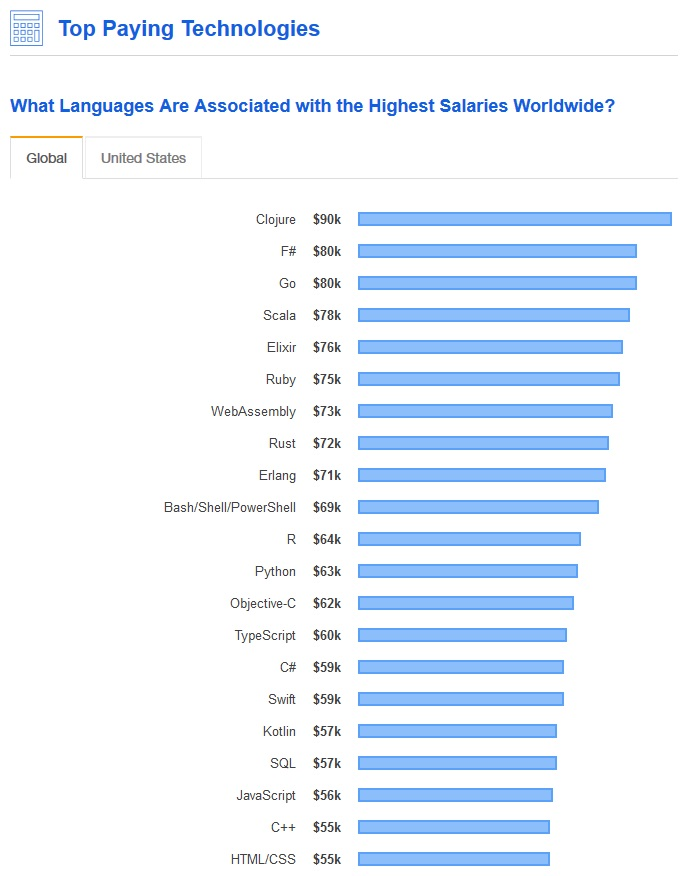
\includegraphics{figs/stackoverflowbestpaid.jpg}
\caption{Fig. 9 a. Salary by programming language}
\end{figure}

    \begin{figure}[H]
\centering
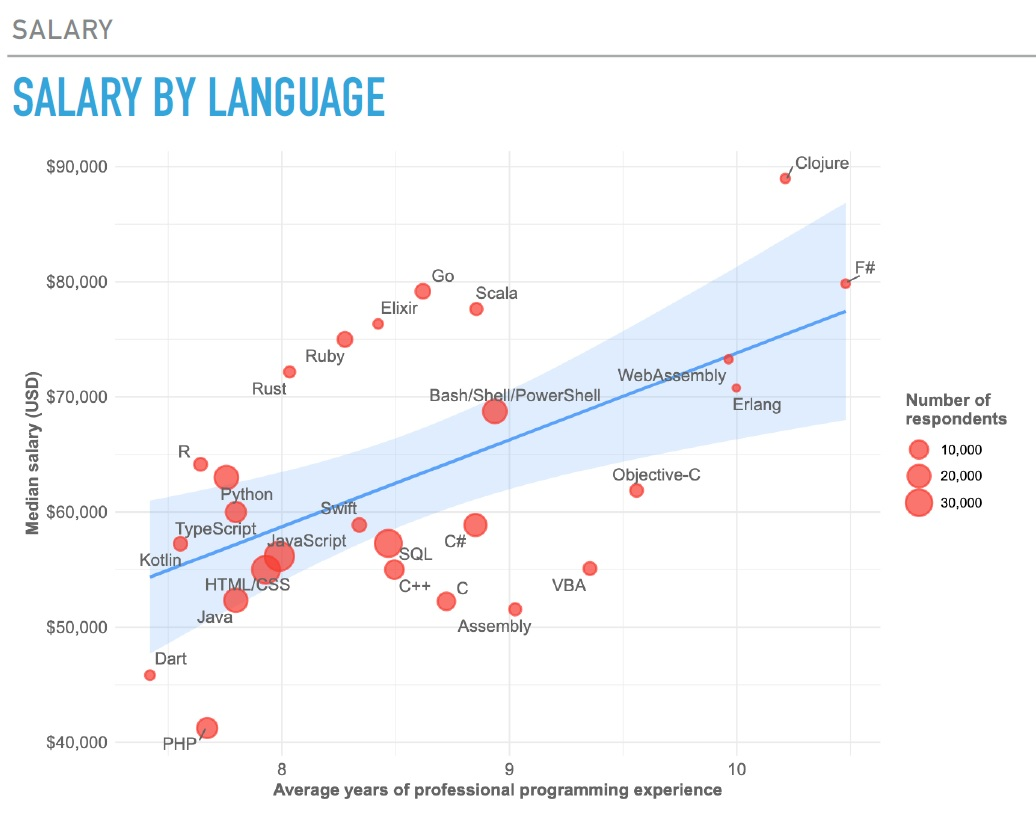
\includegraphics{figs/salarybylanguage.jpg}
\caption{Fig. 9 b. Salary by programming language w.r.t. years of
experience}
\end{figure}

    \hypertarget{installing-python}{%
\section{Installing Python}\label{installing-python}}

    \hypertarget{the-long-and-hard-way}{%
\subsection{The long and hard way}\label{the-long-and-hard-way}}

\begin{enumerate}
\def\labelenumi{\arabic{enumi}.}
\tightlist
\item
  Install Python (https://www.python.org).
\item
  Install a Python Integrated Development Environment (IDE) such as IDLE
  (available when installing Python), Pycharm
  (https://www.jetbrains.com/pycharm/) or Spyder
  (https://pypi.org/project/spyder/).
\item
  Install Jupytor Notebook (http://jupyter.org/).
\end{enumerate}

    \hypertarget{the-fast-way-anaconda-navigator}{%
\subsection{The fast way: Anaconda
Navigator}\label{the-fast-way-anaconda-navigator}}

\begin{itemize}
\tightlist
\item
  Everything can be easily installed using a bundle called
  \href{https://www.anaconda.com/download/}{Anaconda Navigator}.
\end{itemize}

\begin{figure}[H]
\centering
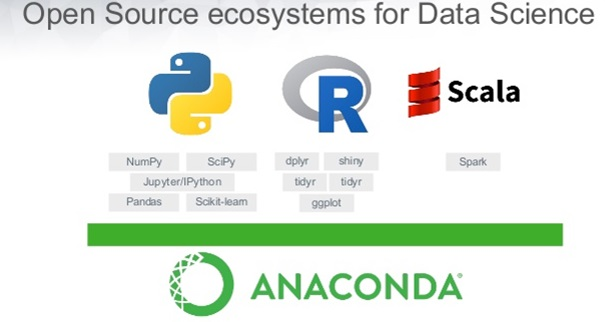
\includegraphics{figs/anaconda.jpg}
\caption{Fig. 10. Anaconda}
\end{figure}

    \hypertarget{how-does-python-look-like}{%
\section{How Does Python Look Like?}\label{how-does-python-look-like}}

    In its most simplistic state, Python acts like a calculator. You simply
write one calculation, and Python gives you the answer!

    \begin{Verbatim}[commandchars=\\\{\}]
{\color{incolor}In [{\color{incolor} }]:} \PY{l+m+mi}{1}\PY{o}{+}\PY{l+m+mi}{1}
\end{Verbatim}


    Moreover, you can also do some coding!

    \begin{Verbatim}[commandchars=\\\{\}]
{\color{incolor}In [{\color{incolor} }]:} \PY{n}{x} \PY{o}{=} \PY{l+m+mi}{2}
        \PY{n}{y} \PY{o}{=} \PY{o}{\PYZhy{}}\PY{l+m+mi}{1}
        \PY{n}{z} \PY{o}{=} \PY{n}{x} \PY{o}{+} \PY{n}{y}
        \PY{n+nb}{print}\PY{p}{(}\PY{n}{z}\PY{p}{)}
\end{Verbatim}


    Notice the simplicity of the Python syntax in the sense that we do not
need to define classes or use a complex and strict structure of
parenthesis!

    \hypertarget{what-else-can-i-do-in-python}{%
\section{What else can I do in
Python?}\label{what-else-can-i-do-in-python}}

    \begin{itemize}
\tightlist
\item
  Python is widely used in \textbf{data science}, as it contains a long
  list of packages that allow importing all kinds of data (i.e.~images,
  sound files, video, spreadsheets, etc.)
\end{itemize}

    \begin{itemize}
\tightlist
\item
  Once data has been imported, you can do some data pre-processing:

  \begin{itemize}
  \tightlist
  \item
    Visualising data of interest
  \item
    Subsectioning rows/columns
  \item
    Augmenting data artificially
  \end{itemize}
\end{itemize}

    \begin{itemize}
\tightlist
\item
  Furthermore, you can perform data analysis and statistics to:

  \begin{itemize}
  \tightlist
  \item
    Understand previous and new trends
  \item
    Predict values of incoming new data
  \item
    Cluster data
  \end{itemize}
\end{itemize}

    \textbf{BONUS:} In fact, this slideshow was done using one of the
numerous Python tools that we have at hand! * I used the \emph{Jupyter
Notebook} integrated development environment (IDE) with an extension
found online called \emph{Rise}.


    % Add a bibliography block to the postdoc
    
    
    
    \end{document}
